\chapter[head={Introduction to language variation and change and history}]{Introduction to language variation and change and history of the English Language}\label{introduction}
% \rohead{Language variation and change and history of the English Language}
\section{The field of Language Variation and Change}\is{language variation and change (field)|(}
Have you ever noticed that your family members, your friends, people you speak with in the street, shops, those you encounter on your travels, or people who speak English in films or on the radio,\is{media} or in fact anyone who speaks English you may have ever listened to or overheard, vary in exactly how they speak English? Have you noticed that some speakers are, for example, more likely to use words such as \emph{dude}, or perhaps that they pronounce certain vowels\is{vowels} differently than you'd expected? Have you ever wondered why linguistic variation exists and just how diverse it could be? Are there limits to language variation, or is literally anything possible? If questions like these intrigue you, you'll be pleased to learn that there's an entire field of linguistics which is concerned with questions of this kind. The field is known as Language Variation and Change, often abbreviated to LVC for convenience. It's a fairly young field, with the \textit{Journal of Language Variation and Change} dating back to 1989 and the seminal work by Weinreich, Labov and Herzog dating back to 1968. Weinreich, Labov and Herzog \citeyearpar[183--7 in particular]{WeinreichLabovHerzog1968} defined the following five problems (or goals) for the theory of language change, which are intertwined and which are seen as central to the researchers working within the field of LVC:
\begin{enumerate}
    \item \textsc{constraints problem}.\is{constraints problem} To begin with, what sort of linguistic variation is there in the world? What sort of language changes are possible? To give a somewhat abstract example, most of us would probably be quite happy imagining two dialects where the vowel\is{vowels} in a word like \emph{kit} was realized as [ɪ] in dialect A but something like [ɛ] in dialect B, i.e. the vowel would be lower\is{vowel lowering} in the latter dialect. (This is actually a change attested in many dialects of English; see \sectref{NC-shifts}.) We would most likely be quite happy with this because all that the speaker needs to do is simply lower the jaw a little bit and produce a vowel of a somewhat lower quality. However, most of us would probably not be so keen on a hypothetical dialect C, in which the vowel\is{vowels} was realized as the plosive [p]. Yes, this would give us [kpt] as the pronunciation of \emph{kit}. But as far as we know, this type of variation and change is not attested. That makes sense: the series of adjustments the speakers would have to make in their vocal tracts would be fairly complex because sounds like [ɛ] and [p] require rather different movements of the bits we use to produce these different sounds (such as different parts of the tongue, etc.). The take-home message is that there \emph{are} constraints on what types of linguistic variation (and thus also language change) are found in the languages of the world.
    \item \textsc{transition problem}.\is{transition problem} When a speaker introduces a new linguistic feature into their language, and thus the language of their community (assuming the community has more than a single speaker!), how does this newly innovated feature spread throughout the community? Does it actually always spread? Let's imagine that one or a couple of random individuals at some point started pronouncing the vowel\is{vowels} in words such as \textit{kit} as [ɛ] rather than [ɪ]. Or that these speakers started glottalling\is{glottalling} their /t/s, thus pronouncing the word \emph{otter} as [ɒʔə] rather than [ɒtə] (also see \chapref{englishtoday}). What happened so that the newly innovated feature (vowel lowering\is{vowel lowering} or glottalling)\is{glottalling} spread at first within the few speakers' community and later possibly across broader geographic areas? And how did it spread across different generations? Was it perhaps the youngest speakers who introduced the two features? Did the subsequent generations simply keep on picking up these new innovative features? All these questions related to how linguistic innovations propagate, get transmitted from one generation to another, and generally spread within a society, fall within what's known as the transition problem.\is{transition problem}
    \item \textsc{embedding problem}.\is{embedding problem} The embedding problem deals with what factors can affect linguistic variation and is thus very similar to the constraints problem.\is{constraints problem} However, the embedding problem focuses on how possible types of language change are affected by various factors. For example, the change from /t/ to a glottal\is{glottalling} stop is not limited to English, so from various languages we know that this change is possible and that we need a language to have a /t/ for this change to be possible to begin with (Constraints problem).\is{constraints problem} But, more specifically back to the embedding problem, when it comes to English, are you more likely to glottal\is{glottalling} your /t/ in words such as \emph{butter} depending on your age? Does it matter where in the word the /t/ is? Would you, say, glottal\is{glottalling} word-medially (\emph{bu\textbf{tt}er}) rather than word-initially (\emph{\textbf{t}abby})? When it comes to a phenomenon like glottalling,\is{glottalling} what social and other factors can possibly affect whether and how a speaker or a group of speakers produce this phenomenon? Understanding the linguistic systems in which we find linguistic variation is crucial for our understanding of how certain features develop in some languages (and their varieties) but not others. This of course also needs to be said of the social aspects of the communities whose members speak the languages in question. Linguistic innovations need to be considered in their linguistic and social contexts.\is{embedding problem}
    \item \textsc{evaluation problem}.\is{evaluation problem} The evaluation problem is all about how the speakers within a community assess, or evaluate, linguistic variation. Sticking to our example of /t/-glottalling,\is{glottalling} do some members of the community perhaps frown upon those who glottal their /t/s? Or does /t/-glottalling\is{glottalling} take place happily without getting noticed by anyone, or indeed fairly happily \emph{despite} being noticed by some? In other words, how do members of a community evaluate this linguistic phenomenon that's been spreading in some varieties of English? 
    \item \textsc{actuation problem}.\is{actuation problem} Finally, why did anyone start glottalling\is{glottalling} their /t/s to begin with? And why did it happen wherever and whenever it did? Why not elsewhere? Why not at another time? Why does a new linguistic feature get introduced in a language at one specific time and in one specific place rather than at some other time and in some other place(s)? This is the most frustrating problem of the field, so much so that some have deemed it unsolvable (see \citealp{StevensHarrington2014} and \citealp{Walkden2017actuation} for overviews). But there's no need to despair -- it's natural that scientists don't have all the answers they would love to have.
\end{enumerate}

\noindent As apparent from the nature of the five problems, LVC overlaps heavily with the aims of two other fields: historical linguistics and sociolinguistics.\is{sociolinguistics} In this book, historical linguistics involves the study of earlier stages of languages and of how languages change. Sociolinguistics focuses on how social aspects interact with language(s). Historical linguistics and sociolinguistics do often overlap in their interest. How does LVC fit in? As we define it, LVC is broader than historical linguistics and sociolinguistics: it encompasses the more traditional and older field of historical linguistics and also embraces that of sociolinguistics.\is{sociolinguistics} 

\begin{sloppypar}
Throughout this textbook, we'll be exploring some of the five problems through the lens of the history of the English language. The most important lesson we'll learn repeatedly is that languages are variable and changing, and as long as there are speakers who use a language, that language is bound to display variation and change. That makes sense: no two individuals are exactly the same in every single respect, though individuals who are socially closer to one another are likely to be more linguistically similar.\is{language variation and change (field)|)}
\end{sloppypar}

In the remainder of this chapter, we'll first discuss concrete examples of what exactly can vary and change when it comes to languages. Because this textbook focuses on the history of the English language (rather than the general principles of language change found in the languages of the world), we'll also introduce you briefly to just how old English is and what historical periods its history tends to be divided into. Finally, we believe it's important for you to realize what good there is in studying something like the history of the English language, and we therefore finish the chapter by giving you six possible reasons (and perhaps you'll think of even more).

\section{What can vary and change in language?}
We can delineate the following linguistic levels: phonetics, phonology, morphology, syntax, lexicon, semantics, and pragmatics. To make sure we're all on the same page throughout our journey, we will now very briefly introduce each of these and illustrate them with examples of linguistic variation. And if you haven't encountered these terms before, worry not -- we explain these below in a nutshell.

\subsection{Phonetics and phonology}\label{phonphon}\is{orthography|(}
Phonetics and phonology represent linguistic levels (and fields) that focus on the sounds of languages. Before we explain the difference between the two, let us get one important message across: letters are not sounds. Please remember this. Letters are not sounds. And one more time, just to make sure: \textit{\textbf{letters}} are \textbf{NOT} \textit{\textbf{sounds}}. How so? If you think of words such as \emph{two} and \emph{too}, the spelling is different (the letters used to spell the two words are not the same), but the pronunciation is \emph{not} different. \emph{Two} and \emph{too} sound the same. We could easily come up with more examples of this type. Although we might think that it would be very handy to have spelling systems that perfectly represent how words are pronounced, this is in fact not what we find in languages with writing systems, for various reasons, and a completely perfect representation may in fact be impractical.\footnote{Even in systems with a one-to-one correspondence between letters and phonemes, much of the fine-grained pronunciation is not reflected in the spelling, such as glottalled\is{glottalling} /t/s or lowered\is{vowel lowering} \emph{kit} vowels!\is{vowels}} 
So, we need to bear in mind that the same letter can correspond to multiple sounds, that a single sound may be represented by a range of letters, and that some letters are not pronounced in English; or they are, but only in some dialects. Let's see an example.

Some of us may be familiar with the fact that most speakers pronounce the words \emph{whales} (large ocean-going mammals) and \emph{Wales} (the small country next to England) as homophones, i.e. their pronunciation is the same (\emph{two} and \emph{too} are also homophones), contrary to what we'd expect based on the spelling. However, the spelling reflects an older stage of the phonological system of English -- there used to be a time when the two words were not homophonous. There are still speakers around, in fact, who distinguish the two words, pronouncing \emph{Wales} as e.g. [wɛɪlz] and \emph{whales} as [ʍɛɪlz], the latter containing a voiceless labiovelar approximant (or a cluster\is{clusters (consonant)} of [h] and [w], depending on the dialect and the analysis you opt for; more on this in \sectref{ME-hdrop}). Discussing letters is therefore NOT the same as discussing sounds.

Now that the distinction between sounds and spelling (or \glossterm{gl-orthography}{orthography}) is clear,\is{orthography|)} let's return to that between phonetics and phonology. If we wanted to be precise, phonetics and phonology would really have to be presented as two different linguistic levels, which are nevertheless closely related. Phonology is preoccupied with abstract sound systems. For example, we know that the words \emph{tuck} and \emph{duck} differ by whether there is a /t/ or a /d/ and nothing else (/tʌk/ and /dʌk/).\is{consonants} Thus, because /t/ and /d/ change the \glossterm{gl-lexicon}{lexical} meaning, these two sounds are \glossterm{gl-phoneme}{phonemes} in English and are of great interest to phonologists. But then on the other hand we find a lot of variation in how exactly different speakers of English pronounce these /t/s and /d/s. Despite this variation, they all preserve the contrast between /t/ and /d/, and again this contrast is at the heart of phonology. Phonetics, on the other hand, focuses (also) on the lexically non-contrastive variation that there is in how we pronounce things. However, there is a considerable overlap between phonetics and phonology, and most phoneticians would also identify as working on phonology.

Finally, before moving on to morphology, let's introduce one term that will come in handy and will be used in this book from now on: \textsc{variant}. In the example above, we saw that there are two ways to pronounce \emph{whales}: with a [w] and with a [ʍ].\footnote{Two ways if we limit ourselves to the discussion surrounding the example given. There is a considerable amount of variation in how speakers may actually phonetically realize what we spell as  <wh> (see e.g. \citealp{Kolísková2016}).} These two ways, [w] and [ʍ], are two variants ([ˈveəɹɪənts]) of realizing what used to be a [ʍ] in earlier stages of the language (see \sectref{ME-hdrop} for the full discussion).\is{consonants}

\subsection{Morphology}\label{morphology}
The field of morphology focuses on the structure of words. For example, standard English would use the -(\emph{e})\emph{s} ending\is{inflection} (a grammatical \glossterm{gl-morpheme}{morpheme}) in the third person singular present tense, as in e.g. \textit{He love\textbf{s} bumblebees}.\is{bumblebees}\is{third person -\emph{s}} In some dialects, though, such as African American English\il{English, African American} (AAE)\footnote{AAE is also known as African American Vernacular English (AAVE) in much of the literature, and sometimes as African American Language (AAL) in more recent work (e.g. \citealp{Lanehart2015}). See \citet[5--8]{Green2002} on the issue of naming this variety. We avoid the term ``vernacular'' where possible here, due to its traditionally \glossterm{gl-pejoration}{pejorative} or negative connotations \citep{Rajendran2019}.} and Cajun English\il{English, Cajun} (spoken in Louisiana, US), there is no -(\emph{e})\emph{s} ending in the third person singular present tense \citep{DuboisHorvath2003}. As we will see in Chapters \ref{OE} and \ref{prehistory}, this could be thought of as a continuation of a change that can be observed throughout the history of the English language, encompassing centuries, since the number of grammatical morphemes present in the English language used to be much higher than today.

\begin{wrapfigure}{r}{0.39\textwidth}
    \centering
    
\includegraphics[scale=0.115]{chapters/img/PrataWala.png}
    \caption{Prata Wala, taken by Míša in Singapore in 2018}
    \label{fig:pratawala}
\end{wrapfigure}

The part of morphology that deals with grammatical morphemes like -(\emph{e})\emph{s} is called \glossterm{gl-inflection}{inflectional}\is{inflection} morphology. It's worth thinking at this point about what we mean when we use the word \emph{word}. In one sense, \emph{loves} and \emph{loved} are different words, but in another sense they are two forms of the same word: you wouldn't look up \emph{loves} or \emph{loved} in a dictionary,\is{dictionaries} you'd look up the verb \emph{love}. When we need to be more precise, we'll say that multiple different \textsc{word-forms} can belong to the same \textsc{lexeme}. The set of word-forms that belongs to a lexeme is called its \glossterm{gl-paradigm}{paradigm},\is{paradigms} and when we need to refer to lexemes specifically we'll adopt the convention of representing them in \emph{ITALIC CAPITALS}. For example, the paradigm of the verb \emph{LOVE} consists of the forms \emph{love}, \emph{loves}, \emph{loved}, and \emph{loving}.\is{paradigms}

\largerpage[2]
Variation in morphology is not limited solely to grammatical morphemes (inflection).\is{inflection} We also find variation in \textsc{word formation},\is{word formation} i.e. the creation of new lexemes. Indian English,\il{English, Indian} for example, uses the morpheme \emph{wallah} `occupation, role, owner'' (\citealp[69]{Kachru1975}; \citealp[362]{Sailaja2012}), as in \emph{the book wallah} `the person who deals with books'', which is not found in other varieties of English. Note that, in morphology just as in phonetics and phonology, spelling\is{orthography} can mislead! \emph{Book wallah} may look like two words on the written page (or on a restaurant sign, as in Figure \ref{fig:pratawala}), but linguists have proposed tests to distinguish stand-alone words from affixes;\is{affixes} for instance, \citet{BresnanMchombo} propose five tests of wordhood. The morpheme \emph{wallah} fails these tests.

Word formation\is{word formation} can involve the addition of an affix\is{affixes} to an independent word, as in this case -- a process usually called \glossterm{gl-derivation}{derivation} -- or it can involve putting together two independent words, usually called \glossterm{gl-compounding}{compounding}. Word formation is a part of language which lives quite happily both within the morphological and the lexical levels. It is not unusual for phenomena to be of relevance to more than a single linguistic level. Thus, morphology also interacts with phonology, and when this happens, the phenomena are both morphological and phonological. If you think of the differences between words such as \emph{sane} and \emph{sanity}, or \emph{serene} and \emph{serenity}, the presence/absence of the morpheme \emph{-ity} is not the only difference.\is{word formation} There are also differences in the quality and the length of some of the vowels:\is{vowels} [sɛɪn] vs. [sænɪtɪ], [sɪˈɹiːn] vs. [sɪˈɹɛnɪtɪ].\is{vowel shortening} As we will see repeatedly in this book, once we start exploring historical aspects of languages, we are bound to come across interactions between different linguistic levels.

\subsection{Syntax}\label{syntax}
\largerpage
Syntax refers to the level of the language that focuses on the structure of phrases, clauses and sentences, above the level of the word. Plenty of variation is found in the realm of syntactic phenomena as well. For instance, \textit{Can meet you at 5.} is something you may be familiar with from text messages or social media.\is{media} This sure looks different from \textit{\textbf{I} can meet you at 5.}, where the subject\is{subjects} is overtly present in the sentence. We do know who the subject is in \textit{Can meet you at 5.} from the context -- the subject\is{subjects} is still very much lurking in the background. Another possible example comes from Welsh English, where we can find what's known as fronting\is{word order} or topicalization, as in Examples (\ref{ex:fronting1}) and (\ref{ex:fronting2}) below (taken from \citealp[158 and 160]{Paulasto2006}).

\begin{exe}
    \ex\label{ex:fronting1} \textbf{Very much involved with [Women's Institute] over the years} I've been.
    \ex\label{ex:fronting2} \textbf{And hens} we had and eggs and ... 
\end{exe}

\noindent Notice that the subject\is{subjects} is preceded by the elements of the clause emphasized in bold, one of which is actually part of the predicate/verb phrase. Fronting does happen in many varieties of English (\textit{\textbf{Pineapples} I really don't like.}), but has been noted to be more frequent in Welsh English\il{English, Welsh} and possible for a more varied set of syntactic elements (see \citealp{Paulasto2006} for more details).

There is a reason why fronting was chosen to illustrate syntactic variation: in fronting, what changes is a movement of a certain unit within a sentence to a different position. The order of words\is{word order} and constituents falls squarely within the syntactic realm. But sometimes it may not be quite so obvious that the level of language we are dealing with is that of syntax. For example, in most varieties of English, there can only be a single modal\is{modals} within a clause, so that the following sentences would not be grammatical (taken from \citealp[17--18]{Bour2015}):

\begin{exe}
    \ex\label{ex:mightcould} He'\textbf{ll might could} do it for you. \hfill (Hawick, Scotland)
    \ex Sorry, we don't carry them anymore, but you know, 
    you \textbf{may might can} get one right over there at Wicks. \hfill (North and South Carolina)
\end{exe}

\largerpage
\noindent But there are nevertheless dialects of English\is{regional variation} where these multiple modals\is{modals} can be found (such as those in North and South Carolina, Tennessee, Arkansas, the Appalachians and the Ozark territories, Southern Scotland, Northern England, and North-Eastern Ulster; \citealp[14]{Bour2015}, \citealp{Huang2011}).

This type of variation is not, strictly speaking, only about the word order.\is{word order} There is also something about the nature of the specific verbs involved which makes this type of variation of interest to those who focus on the \glossterm{gl-lexicon}{lexicon} (for example, are all of these modal\is{modals} verbs really verbs, or could some of them be classified as adverbs, or even something else?), and notice that the modal \emph{will} is also phonologically reduced in (\ref{ex:mightcould}). Many phenomena that are syntactic in nature could thus often be seen as falling within the remit of morphology, and even phonetics and phonology, as well. Another example of this in English dialects would be related to negation.\is{negation} When we contrast \textit{\textbf{Will he not} do it for you?} with \textit{\textbf{Won't he} do it for you?}, not only is there a difference in whether the negative\is{negation} marker precedes or follows the subject,\is{subjects} but the phonology and thus also the word structure of the verb \emph{will} is also affected. Phenomena which are both morphological and syntactic can be said to fall within the area of morphosyntax.

When thinking about the syntax of different varieties of English, it's useful to think about the words of the language as being attached to an abstract structure of a sentence, as in (\ref{ex:treediagram}).\is{syntactic trees} You can think of the words themselves as the skin on the bones of a skeleton (i.e. the abstract structure), or the leaves on a tree. In fact, \textsc{tree diagram} is the usual term for diagrams like (\ref{ex:treediagram}).\is{syntactic trees}

\begin{exe}
    \ex \label{ex:treediagram}
    \Tree [.IP \textit{We} [.I$'$ [.I \textit{can} ] [.VP [.V \textit{meet} ] \textit{you} ]]]
\end{exe}

\noindent In this view of syntax, sentences are made up of hierarchically structured phrases. The tree structure here includes a Verb Phrase -- VP -- and an Inflection\is{inflection} Phrase -- IP. Each phrase has a \textsc{head}: V (the verb) for the VP, and I for the IP. Phrases may also have a \textsc{complement} (the sister of the head) and a \textsc{specifier}. In most present-day English varieties, we can say that the subject\is{subjects} (here, \emph{We}) is in the specifier of IP and that the object (here, \emph{you}) is in the complement of VP.\is{syntactic trees}


\begin{syntaxbox}{X-bar theory}
\is{syntactic trees}\is{X-bar theory}
We can talk about elements of a syntactic tree having mothers and sisters, like in a family tree: so, the verb \emph{meet} is the sister of \emph{you} in Example (\ref{ex:treediagram}), and their mother is the VP element itself. If a phrase has a specifier, then the specifier's sister will be something that is neither a head nor a full phrase, but something in the middle: in Example (\ref{ex:treediagram}), this is I$'$ (or ``I-bar''). It's the mother of I and VP, the daughter of IP, and the sister of the subject\is{subjects} \emph{We}. This approach to syntax is called X-bar theory, and it's quite widely assumed. In this book we'll keep the syntactic theory to a minimum, but if you'd like to pick up some more background, \citet{Carnie2013} is a good place to look.
\end{syntaxbox}

\noindent Sometimes, syntactic variation will involve words appearing in different places in the tree while the abstract structure may stay the same. In spring and autumn, the leaves of trees may come and go, but the tree's trunk and branches don't change much. Sometimes, we'll argue that the tree structure itself changes; over its long life, the branches of a tree may move, and new branches may be grown. What's exciting about syntactic change is establishing the limits of variation. Which aspects of syntax are universal to human cognition, and which can vary cross-linguistically? Studying the history and varieties of English can shed light on these questions.\is{syntactic trees}

\subsection{Lexicon}\label{lexicon}
We have already seen an example of variation in word formation\is{word formation} -- the \emph{wallah} example -- and said that variation in word formation can also be viewed as pertaining to the level of the \glossterm{gl-lexicon}{lexicon} (\sectref{morphology}). Indeed, word formation is all about expanding the lexicon. But morphological word formation\is{word formation} is not all there is to this linguistic level. Semantics is also important, and variation can be found regarding, for example, what word X means in dialect A as opposed to dialect B, and what words are used for idea Z in which dialect. Let's see some examples to make this less abstract.

Speakers of Singapore English\il{English, Singapore} would use \emph{café} to refer to a place to eat (so a bistro) rather than a place to have a coffee (and typically some sort of cake), as illustrated in Figure \ref{fig:boonlaycafe}.\footnote{That \emph{café} is indeed used with a different meaning in Singapore English has been confirmed by Gerry Kwek,\ia{Kwek, Gerry} a local Singapore linguist (personal communication, 2018).}

\begin{figure}[H]
    \centering
    
\includegraphics[scale=0.2]{chapters/img/boonlaycafe.png}
    \caption{A typical café in Singapore, selling mainly savoury take-away meals (taken by Míša in 2018)}
    \label{fig:boonlaycafe}
\end{figure}

\noindent Where speakers of American English\il{English, American} would use \emph{pants}, most speakers of British English would use \emph{trousers}.\footnote{Although see \url{https://www.ourdialects.uk/maps/clothing/}.} And a small bread-like consumable can be referred to with a range of terms, such as \emph{bap}, \emph{barm}, \emph{batch}, \emph{bun}, \emph{cob}, \emph{muffin}, \emph{roll}, \emph{tea cake}, and possibly more, just within the UK.\footnote{Find out more about the linguistic wonders of small bread-like consumables here: \url{https://www.ourdialects.uk/maps/bread/}.}

Lexical variation is by no means limited to nouns. Thus, where some speakers of English may say \textit{You \textbf{ought to} know this}, others may say \textit{You \textbf{should} know this}. Lexical variation is probably the first type of language variation we think of, but as we have seen by now, the other linguistic levels by no means escape variation and change.

\subsection{Pragmatics/discourse}\label{pragmatics}\is{historical pragmatics|(}
Pragmatic aspects of language are those that are related to the context in which conversation takes place. This can be linguistic context, situational context, and social context \citep{BergmannHallRoss2007}. Right now and right here, we don't need to worry about the different types of contexts that there are -- what matters is that pragmatics looks at units of language \textit{in context} rather than in an abstract vacuum (like we've been doing thus far in this chapter when throwing examples at you). Some of you may have come across the term \textsc{discourse} as well. Usually, discourse is defined as language use and linguistic structure beyond the level of the sentence. What discourse and pragmatics are really about is how the whole communication process happens, and this requires various aspects of language to be considered. For this reason, phenomena from various other linguistic levels could easily fall within the scope of pragmatics. It's time for some examples now.

We find abundant variation at the pragmatic and discourse-related level. The Tyneside area of the UK is well known for using terms of endearment such as \emph{pet} to address another speaker \citep[346]{Beal2000}.\is{regional variation} It's true -- Míša was once making her way to Gateshead from the airport at Newcastle, when the lady who sat right opposite her, a complete stranger, asked, ``What are you down for, pet? Holidays?'', and she knew she was in Tyneside. And in the Midlands of England, where George grew up, \emph{duck} (a term normally used for an aquatic bird\is{birds} in most varieties of English) is used as a term of address. Addressing a stranger as \emph{pet}, \emph{love}, or \emph{duck} would hardly be appropriate in all English-speaking regions of the world.\is{regional variation} Some other good examples demonstrating the importance of context would be \textit{Oh fudge, my hair is on fire!} and \textit{Dear me, did he kidnap the baby?} (taken from \citealp[50]{Lakoff1973}). Here, we see a mismatch between the gravity of the situation (hair being on fire, a baby being kidnapped) and the exclamations that are not considered appropriate in such contexts (\textit{oh fudge}, \textit{dear me}).

An example of a phonetic phenomenon with a range of pragmatic functions would be voice quality. Do you, for example, change something about your voice depending on the context? Do you whisper if you want to signal secrecy? The beauty of pragmatics, and probably the frustrating thing about it (depending on your perspective), is that any aspect of language can potentially have a pragmatic function of some sort, and contribute to the structure of the whole conversation.\is{historical pragmatics|)}

\section{The field of History of the English Language}\label{field-HEL}
As the name suggests, the field of History of the English Language is concerned with the history of the English language. This includes any linguistic level you could think of, which makes a subject like this somewhat more challenging and wide-ranging than those subjects which limit themselves to specific linguistic levels. Studying the history of the English language (or any other language, for that matter) is a holistic approach to understanding how languages work. And that's worth the effort.

Depending on which textbook and which article you pick, you will find different estimates as to when English was born, so to speak. Some authors give the year 449, while others mention the 7th century CE, and yet others would go back still further (see \sectref{history-and-context} for some discussion). If we decide to be on the safe side and say that we'll consider English to have begun in the 7th century, which is the earliest that any texts written in English have been preserved, and stop in 2022, which is when this book was published, we end up with an amazing 15 centuries. All the examples illustrating different types of variation presented in this chapter are only the tip of the iceberg of the variation we could possibly discuss when it comes to the 20th and the 21st centuries. We could very easily have several courses on the topic, limiting ourselves just to these two centuries. But you're taking a course on the history of the English language, so it's important that we bear in mind that the amount of variation and number of changes to cover is bound to be substantial, simply because of the time involved. And that's exactly why we have to be selective in which aspects from different periods of the language we present to you in the following chapters. If we thereby leave out some of your favourite linguistic phenomena, we're sorry! But we hope to also give you the tools to find out more about other changes in the history of English, using your own initiative.

The history of the English language is typically divided into the following periods:

\begin{itemize}
    \item \begin{tabular}{p{4cm}p{2cm}l}
    Old English & OE & 600--1150\end{tabular}
    \item \begin{tabular}{p{4cm}p{2cm}l} 
    Middle English & ME & 1150--1500\end{tabular}
    \item \begin{tabular}{p{4cm}p{2cm}l} 
    Early Modern English & EModE & 1500--1700\end{tabular}
    \item \begin{tabular}{p{4cm}p{2cm}l} 
    Late(r) Modern English & LModE & 1700--1945\end{tabular}
    \item \begin{tabular}{p{4cm}p{2cm}l} 
    Present Day English & PDE & 1945--present\end{tabular}
\end{itemize}

\noindent The Old English and the Middle English periods can also be further divided into Early Old English and Late Old English, and Early Middle English and Late Middle English periods. Right now, in this chapter, it's not important to discuss when exactly each period can be said to begin and end -- we'll take this on in the chapters that follow. What is nevertheless important to realize is that there are multiple ways in which we can ``slice up'' the history of English into these periods. For example, we could use important historical events to mark the beginning/end of the periods, such as the Norman Conquest\is{Norman Conquest} (see \chapref{ME}). Or we could look at the linguistic structure of the language across different centuries and suggest that a new period starts because that's when we can see a significant linguistic difference in contrast to the previous centuries. However, neither of these approaches is without its problems. Although sociocultural changes are often reflected in the language(s) of the societies in question, this can happen in various ways, some of which are more subtle than others. Furthermore, we'll also see in various parts of this book that often linguistic change may take centuries; in other words, linguistic change takes time and is not necessarily as sudden as we may expect at first. In sum, any periodization of the history of a language is an idealization, because languages don't change overnight and resist being chopped up into discrete historical chunks.

Another important thing to remember about the history of English is just how interdisciplinary it can be. We approach the history of English from a linguistic perspective; however, it necessarily overlaps with fields other than linguistics. The most obviously overlapping field is that of history (which is in itself a fairly broad field with many different subfields), but we will see that the subject can be approached also from the perspectives of archaeology\is{archaeology} (\chapref{prehistory}), literature (all chapters), and media\is{media} studies (\chapref{englishtoday}), among others. This aspect of the history of English makes studying it a thrilling endeavour, though admittedly to some of us perhaps also a somewhat terrifying one. But rest assured -- no one could possibly know everything that there is to know about the history of the English language, including the teachers, and we certainly don't expect you to!

\section{Why study History of the English Language?}
The most obvious reason to study the history of the English language is to understand how English has changed ever since it came into existence. However, the benefits of studying the history of the language are manifold and deeper than simply gathering facts about how English has been changing and when. We review six of those benefits in what follows.

\subsection{Variation, variation everywhere}\label{variation}
It is astounding just how much linguistic variation surrounds us without us even noticing, at least consciously. When we study a subject such as the history of English, we necessarily focus on how language changes. Change, however, cannot happen without there being variation first. This means that approaching the history of any language includes approaching linguistic variation. Irrespective of which language(s) we speak, studying the linguistic variation in this language or these languages enables us to discover intriguing social and interpersonal patterns that affect all of us, on a daily basis. We've seen plenty of examples relevant for English in \sectref{field-HEL}, but more examples are coming in \chapref{englishtoday}, where we discuss the main trends in how Present Day English has been changing. Where does all this variation come from? How did it come about? What functions does it have? What purpose? If you're interested in these questions, then you're also interested in the history of the English language, and Language Variation and Change more generally. Doing a course on the history of the English language will provide you with some concrete examples linked to these questions.

\subsection{Irregularities}\label{irregularities}\is{irregularities|(}
Those of us who are not native speakers of English will know that English is full of irregularities we are expected to tackle. For example, most verbs form their past tense by adding -(\emph{e})\emph{d} to their root: \textit{I love bumblebees. And when I was 7 I also lov\textbf{ed} bumblebees}.\is{bumblebees} But, in standard English at least, we can't say \textit{I sing only when I'm alone, and when I was 7 I also sing\textbf{ed} only when I was alone}.

We're also expected to learn that although the plural\is{plurals} of \emph{dog} is \emph{dogs}, the plural of \emph{sheep} is ``simply'' \emph{sheep}. Or that whilst the noun \emph{use} is pronounced as [juːs], the verb \emph{to use} is pronounced as [juːz]. And there's more irregularities of this type. If you intend to teach English as a foreign language (EFL), or English to speakers of other languages (ESOL), your life will be full of facing these irregularities in one way or another. Where do they come from? This is the sort of question we can't answer unless we delve into the study of the history of the English language!\is{irregularities|)}

\largerpage[-1]
\subsection{Interpreting older literary and other texts written in English}\label{interpreting-older-texts}
Some of you may be interested primarily in history, which means you may need to work with older documents, such as decrees and other legal works.\is{legal language} If you are interested in such legal documents, these could come down to us from different points in time (10th century, 15th century...). Here's an example from a 15th-century private charter:\footnote{This extract is taken from the \glossterm{gl-corpus}{Corpus}\is{corpora} of Middle English Prose and Verse, 2006,  \url{https://quod.lib.umich.edu/cgi/t/text/text-idx?c=cme;cc=cme;view=toc;idno=AJD3529.0001.001}}

\begin{exe}
    \ex In þe weche thyng wytnes to thys presont chertar I haue put to my sele, be thes wetnessys, \&c.\\
    Literally: In the which thing witness to this present charter I have put to my seal, by these witnesses, etc.
\end{exe}

\noindent This is probably not the easiest text to understand -- in part because of the style specific to legal documents,\is{legal language} but in part no doubt because of the differences between 15th-century English and Present Day English. You may object -- surely someone must have translated all these older texts, so why bother with understanding 15th-century English? Indeed, translations do exist, but how much has been changed and lost in translation? Unless you can tackle the original texts, you will never know...

Or perhaps you are keen on literature, and/or perhaps you are interested in gender studies.\is{gender studies} If this is the case, you may be interested in the Old English elegy called \textit{Wulf and Eadwacer}. Here's just one line:\footnote{This extract is taken from \textit{The Exeter Book}, London, Exeter Cathedral Library, MS 3501, \emph{Wulf and Eadwacer}, 100v-101r \url{https://www.bl.uk/collection-items/exeter-book}. You can find the full text in \sectref{OE-wulf}.}

\begin{exe}
    \ex willað hy hine aþecgan gif he on þreat cymeð\\
    Literally: will they him take if he on troop comes
\end{exe}

\noindent Hmm, that's probably even worse than the English from the 15th century. Again, translations into the English of today do exist, but unless you can engage with the original text, you won't know how much has been altered in the process of translation. For example, Faulkner's\ia{Faulkner, William} \emph{Light in August} uses a range of dialectal features in the English original, which -- to Míša's horror -- were completely lost in the \ili{Czech} translation she'd read. That's not something you want to discover after reading about 400 pages you intend to engage with from an analytical point of view, albeit a primarily literary one.

Taking a basic introduction to the history of the English language will enable you to engage with texts written in older forms of the language, even if your primary interests lie in areas other than linguistics. The history of the English language can therefore provide you with a useful tool even if you're not linguistically-oriented.

\subsection{The social life of language}\label{social-life}
William Labov\ia{Labov, William} is often considered the founding father of sociolinguistics\is{sociolinguistics} (see \citealp{Koerner1991} for the importance of Labov's work within LVC) and yet he refused to use the term sociolinguistics for a long time (see for example \citealp{Chambers2017}). This is because, for Labov, language is very much a social thing: how can we ever reach a full understanding of how language works and functions if we do not consider social factors? As long as languages are spoken and written by living human beings, there will be variation which reflects at least some of the social variation of the speakers involved. This is not to say that linguistic phenomena are always only affected by social aspects of our lives -- not at all. But the social aspects of our lives do play an important role. Let's think of our \textit{He love bumblebees}\is{bumblebees} example from above.

In Cajun Vernacular English\il{English, Cajun} (spoken in Louisiana), age and education level affect the frequency\is{frequency} at which 3rd-person singular -\emph{s}\is{third person -\emph{s}} applies \citep[39]{DuboisHorvath2003}, i.e. how frequently we actually find it where it occurs in standard Englishes. This grammatical morpheme is reported to be absent in 32\% of the speakers studied by \citet[42]{DuboisHorvath2003} on average, whereas this absence reaches only 14\% in Devon English\il{English, Devon} \citeyearpar[42]{DuboisHorvath2003}. Region\is{regional variation} is therefore another factor which affects variants in more and less subtle ways. Importantly, in these cases, we're not dealing with either-or differences in the sense that one group of individuals either uses a certain variant all the time or never does. What's typical of variation around us is just how gradient it often is. Thus, variation is indeed everywhere, but it may manifest itself in fairly subtle ways. Social aspects of speakers can therefore correlate with linguistic variation. 

\citet[212 and 223]{Labov2010} presents us with an example of how ideological disagreement may possibly motivate why the vowel\is{vowels} system of the linguistic Inland North\il{English, Inland North} in the USA (something we will return to in \chapref{englishtoday}) has been developing differently from that of the West Midlands.\il{English, Midwest} He shows that the residents of the Inland North\is{regional variation} (as opposed to those from North and Midwest) were responsible for most of the votes for John Kerry, the Democratic presidential candidate, in 2004 -- and this is considered to reflect the political differences between Americans from the Inland North and the Midwest, similarly to the linguistic variation found in their vowel\is{vowels} systems.


\begin{peoplebox}{William Labov}
The importance of the American linguist William Labov\ia{Labov, William} (1927--) can't be overstated. Labov has shown that there is order in variation, i.e. that variation in language is not haphazard. He has also made a persuasive case that speakers of non-standard varieties of English do not have slower learning abilities than those of standard English\is{standardization} (in the 20th and 21st centuries this has been particularly important for the African American community, but of course is also applicable much more widely). Labov has also proposed new methodological practices, aiming to reflect different degrees of attention the speakers pay to speech when observed. You can listen to Labov's lecture titled \emph{A life of learning: six people I have learned from} here: \url{https://vimeo.com/70455840} 
\end{peoplebox}


\noindent Understanding just how exactly social factors interact with linguistic phenomena is something which is of interest to those who enjoy linguistics as well as history, society, and culture. The linguistically-minded will be interested in general principles of language variation and change. The sociohistorically-minded can use certain linguistic variants and changes as a tool rather than a primary object of interest. We will see many examples of linguistic changes linked to social changes throughout the history of the English language, in each of its periods, as we move backwards in time in the remaining chapters of this book.

\subsection{Different linguistic levels can interact}\label{linguistic-interaction}
Different linguistic levels can interact! Indeed, you've seen some evidence thereof when we had a look at examples that don't straightforwardly fall within a single level of language. Interactions between different linguistic levels can be seen rather nicely through the lens of language change. But let's see an example which is really relevant for all the linguistic levels:

\begin{exe}
  \ex \begin{xlist}
    \ex I \emph{am going} to town later today.
    \ex I \emph{am going to} go to town later today.
    \ex I'\emph{m going to} go to town later today.
    \ex I'\emph{m gonna} go to town later today.
    \ex I'\emph{m going to} meditate later today.
    \ex I'\emph{m gonna} meditate later today.
    \ex I'\emph{ma} meditate later today.
  \end{xlist}
\end{exe}

\noindent Much could be said about which linguistic levels interact with which and how exactly here. But let's discuss only the most obvious interactions. We can imagine that as one speaks faster in for example conversation with friends rather than when reading these sentences out loud from this page, we may not pronounce every single sound of \textit{am going to}\is{grammaticalization} (You can also think of \textit{I don't know} being pronounced as [aɪdənəʊ] `I dunno' rather than [aɪ dəʊnt nəʊ]). Many would most likely say \textit{am gonna}, or some such. This is about sounds, but not only -- what happened to the \emph{to}? What happened to the -\emph{ing} morpheme? And do all of these different forms mean the same? If you think about it, although we can say \emph{I'm gonna meditate} (at some point in future),\is{futurity} we can't say \emph{I'm gonna town} (meaning `I'm going to town'). This is because there are actually two \emph{GO} verbs in English, pronounced in a very similar way. One of these verbs indicates motion, whilst the other one refers to a future event -- they are semantically different, and this is also reflected in their pronunciation. Historically, the future \emph{GO} comes from the motion \emph{GO}, something we'll discuss in \chapref{LModE}.\is{futurity} This is an example of \glossterm{gl-grammaticalization}{grammaticalization}\is{grammaticalization} -- the historical process by which lexical words (like the \emph{GO} of motion) become grammatical, closed-class words (like the semi-modal\is{modals} \emph{gonna}), and free words become bound morphemes (often through an intermediate \glossterm{gl-clitic}{clitic}\is{clitics} stage). Grammaticalization is very common in language change in general (see \citealp{HopperTraugott2003}) and in the history of English in particular, and we'll see many examples throughout the book.\is{grammaticalization}

\subsection{Language change is inevitable (and perfectly normal)}
You may have come across the opinion that language change is bad -- the way teenagers speak these days, and so on. However, language change is not only perfectly normal but actually inevitable. This is because social differences within communities are also inevitable, however subtle, and language changes whenever society changes. As we will see in Chapters \ref{LModE} and \ref{EModE}, the variety of language which gets to be established as the standard one within the relevant community has nothing to do with the linguistic properties of such varieties. What matters in such cases is the hard-to-predict result of a number of intertwined socio-historical events. We can discuss Standard British English and Standard American English today, but there were times when the notion of a (standard) variety of American English was rather novel.\is{standardization} Today many dialects of English are deemed ``incorrect'', simply because they diverge from the dialects that have happened to ``make it'' into the social elite of standard dialects. But it is important to realize that standard Englishes are just some of the many different dialects of English (see \citealp{Trudgill1999}). A history of English is a history of all of these varieties, not just standard Englishes.

Sometimes, we're rather sad to say, discrimination and bullying can take place depending on one's native dialect (and often other characteristics). The Accentism\is{accentism} Project (Carrie\ia{Carrie, Erin} and Drummond)\ia{Drummond, Rob} is full of testimonials of linguistic discrimination from a range of users of English.\footnote{For more, go to the project's webpage: \url{https://accentism.org/}. For even more, \citet{Paterson2019} is an accessible interview with the project's founders.} The work of linguists doing research within the field of LVC can help communities: for instance, \citet{Labov1966} has demonstrated that, contrary to the opinions of the time, African American English\il{English, African American} is governed by linguistic rules, just like any other variety of English (such as Standard American English),\il{English, American} and should not be considered a sign of lower intelligence and slower learning.\is{accentism}

All varieties of English are subject to variation and change. Which variety happens to be selected as the standard\is{standardization} one is similarly subject to change too. This is something we will see as we look into the history of the English language in more detail across the centuries (Chapters \ref{LModE}--\ref{OE}, especially \sectref{EModE-standardization}).\is{standardization}

\section{Final note}
We hope you'll find that the history of the English language is an intriguing subject to study and that you'll join us on this fascinating ride. The exercises below will further help you reflect on the topics discussed in this chapter.

\addsec{Suggested exercises}

\begin{exercises}{The Sower and the Seed}\label{sower-and-seed}
The Christian\is{Christianity} Bible is a particularly useful text for the study of language change, because it's been translated so many times into so many different languages over the centuries. Below are four versions of the Parable of the Sower and the Seed (Matthew 13, verses 3--4), from different points in time, across a thousand years of the history of English.

\begin{itemize}
    \item \textit{A farmer went out to sow his seed. As he was scattering the seed, some fell along the path, and the birds\is{birds} came and ate it up.}\\ 
	(New International Version, 1973)
    \item \textit{Behold, a sower went forth to sow; And when he sowed, some seeds fell by the way side, and the fowls came and devoured them up.}\\ 
	(King James\ia{Stuart, James (King James I)} version, 1611)
    \item \textit{Lo! he that sowith, yede out to sowe his seed. And while he sowith, summe seedis felden bisidis the weie, and briddis of the eir camen, and eeten hem.}\\
	(Wycliffe\ia{Wycliffe, John} version, c. 1395)
    \item \textit{Soþlice ut eode se sædere hys sæd to sawenne and þa þa he seow. sume hig feollon wiþ weg. and fuglas comun and æton þa;}\\
    (West Saxon\il{Old English, West Saxon} Gospels, c. 990)
\end{itemize}

\noindent The fourth and oldest version will probably be difficult for you to read right now. But don't worry -- we'll get there by \chapref{OE}! For now, try to identify differences between the texts in terms of each of the linguistic levels we've discussed in this chapter:
\begin{itemize}
    \item Phonetics \& phonology\\ 
    (hint: here you'll need to make an educated guess, based on spelling)\is{orthography}
    \item Morphology
    (hint: look at the verbs in the Wycliffe version!)
    \item Syntax\\
    (hint: what's different about the clause ``As he was scattering the seed'' in the New International Version that isn't found in any of the earlier versions?)
    \item \glossterm{gl-lexicon}{Lexicon}
    \item Pragmatics/discourse
\end{itemize}
\end{exercises}

\begin{exercises}{Jabberwocky}\label{jabberwocky}\is{poetry|(}
Here are extracts from Lewis Carroll's\ia{Carroll, Lewis} \emph{Jabberwocky} (1871):

\begin{center}
'Twas \textbf{brillig} and the \textbf{slithy toves}\\
Did \textbf{gyre} and \textbf{gimble} in the \textbf{wabe};\\
All \textbf{mimsy} were the \textbf{borogoves}\\
And the \textbf{mome raths outgrabe}.\\
 
‘Beware the \textbf{Jabberwock} my son!\\
The jaws that bite, the claws that catch\\
Beware the \textbf{Jubjub} bird,\is{birds} and shun\\
The \textbf{frumious Bandersnatch}!'\\

And, as in \textbf{uffish} thought he stood,\\
The Jabberwock, with eyes of flame,\\
Came \textbf{whiffling} through the \textbf{tulgey} wood,\\
And \textbf{burbled} as it came!\\
\end{center}

\noindent For each of the words in bold, answer the following questions:

\begin{enumerate}
    \item What word class (e.g. adjective, noun, verb...) would you suggest each of the words belongs to and why?
    \item Where the word has an affix\is{affixes} (e.g. \emph{-ed}), can you think of any other English words that also have this affix?
    \item Almost half of the words in the first stanza are not English words (or weren't when Lewis Carroll wrote them). Does that mean the poem is still written in English? Explain your answer.
\end{enumerate}

\noindent \emph{Tip for teachers}: Question 3 can be used for a written exercise.\\

\noindent \emph{Tip for teachers}: You could also use the following question if your students are familiar with open and closed classes: Do the words in bold belong to closed or open classes?\\  

\noindent \emph{Acknowledgement}: The questions are adopted and adapted from Johanna Wood's\ia{Wood, Johanna L.} \emph{Jabberwocky} exercise, passed down to us in 2017.\is{poetry|)}

\end{exercises}

\begin{exercises}{Practice with trees}\label{exercise-syntax}

Look at the following tree.\is{syntactic trees}\is{bumblebees}\\

\qtreecentertrue \Tree [.IP \textit{Everyone} [.I$'$ [.I \textit{should} ] [.VP [.V \textit{appreciate} ] \textit{bumblebees} ]]]


\noindent Try to answer the following questions based on the terms and notions introduced in \sectref{syntax}.

\begin{enumerate}
    \item What word or phrase is in the specifier of IP?
    \item What word or phrase is in the complement of VP?
    \item What word or phrase is in the head of IP?
    \item What word or phrase is in the complement of IP?
    \item What is the mother of I$'$?
    \item What are the daughters of I$'$?
    \item What is the sister of the object \emph{bumblebees}?\is{syntactic trees}\is{bumblebees}
\end{enumerate}

\end{exercises}

\begin{exercises}{Variation at which linguistic level?}\label{exercise-variation}\is{standardization|(}
Look at the following sentences, and provide what you think are their Standard English equivalents (where applicable). Then answer the questions that follow the examples.\il{English, Welsh}\il{English, Tyneside}
\begin{itemize}
    \item[A.]\textit{So from where do you come from?} [Aberystwyth, mid Wales]
    \item[B.]\textit{Yes, it has changed, but I still do come across it.} [Aberystwyth, mid Wales]
    \item[C.]\textit{I dunno, people kind of associate Newcastle wi like sort of rougher people sort of thing, you know.} [Berwick-upon-Tweed]
    \item[D.]\textit{How would I change the world? That's a simple question.} [Aberystwyth, mid Wales]
    \item[E.]\textit{In the seventies when I was in school, I was sort of you know laughed upon.} [Aberystwyth, mid Wales]
    \item[F.]\textit{I divvent know nowt else you know.} [Tyneside]
    \item[G.]\textit{They said I was too clever, they went and jumped us two classes, and I was never no good after that.} [Tyneside]
    \item[H.]\textit{So they hadn't any time for anyone getting on in years.} [Tyneside]
    \item[I.]A photo Míša took at the train station in Newcastle, Tyneside, in 2016:
    \begin{figure}[H]
        \centering
        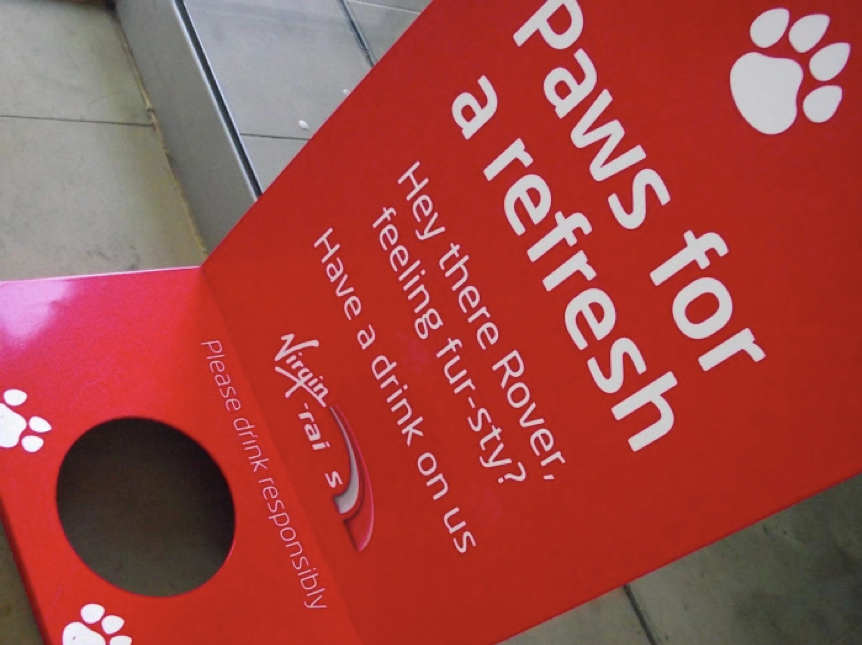
\includegraphics[scale=0.3]{chapters/img/Paws_for_a_refresh.png}
        \label{fig:paws}
    \end{figure}
\end{itemize}

\begin{enumerate}
    \item Are there any sentences which contain no non-standard features? Which ones?
	\item What are the non-standard features found in the other sentences?
    \item Which linguistic level (e.g. phonetics \& phonology, syntax...) do these features belong to, would you say?
	\item Are the non-standard features restricted by region,\is{regional variation} formality, or possibly anything else?
\end{enumerate}

\noindent The sentences are taken from \citet{BealCorrigan2005}, \citet{PichlerLevey2010}, and M\'{i}\v{s}a's corpus\is{corpora} of English recorded in Aberystwyth, Wales.\footnote{Now available here: \url{https://osf.io/2vpgr/}, through combined efforts with Kamil Ka\'{z}mierski.}\\ 

\noindent \emph{Acknowledgement}: This exercise was inspired by some of Heike Pichler's\ia{Pichler, Heike} materials from her Language across Space course at Newcastle University (2014, 2016).\is{standardization|)}
\end{exercises}

\begin{exercises}{Whence and w(h)ither variation?}
\chili{}

Think about some examples of language variation in English that you have noticed (e.g. when watching films in English, in your classes, when reading this book or some other books, or when speaking with friends and family).
\begin{itemize}
    \item [A.] Why do you think this variation exists?
    \item [B.] Is it possible to prevent this variation from 
    happening? Why (not)?
\end{itemize}

\noindent Note that these are open-ended questions and many different answers are reasonable.\\

\noindent \emph{Tip for students}: If you want to follow up on these topics beyond the seminar discussion, read \citet[chapter 1]{Aitchison2012}.\\

\noindent \emph{Tip for teachers}: This exercise can be used as a written exercise.

\end{exercises}

\begin{exercises}{Claims about linguistic variation}
\chili{}

Imagine a situation in which someone above 60 years of age complains\is{complaint tradition} to a friend about how the youngsters today don't know how to speak English properly. Indeed, it seems that English is going to the dogs...
 
Within 300 words, explain how you would establish whether this claim is or isn't correct. More specifically, introduce the claim tested, then suggest the types of evidence you would use. Be critical of the types of evidence available and their advantages and disadvantages.\\
 
\noindent \emph{Tip for teachers}: Using group blog entries or wikis for this assignment as well as a reasonable deadline is a good idea -- it saves time for both the students and you, and the deadline will allow you to go through the contributions prior to the seminar.\\
 
\noindent \emph{Tip for teachers}: Add a condition of the students having to use at least 1 source (or more) to back up their claims, using the reference style of your department.\\
\end{exercises}

\begin{furtherreading}
Is your linguistic terminology a bit rusty? You can find some key terms in our \hyperref[glossary]{glossary}. Beyond that, David Crystal's \textit{Dictionary of Linguistics and Phonetics} \citeyearpar{Crystal2003a} is an excellent rust remover. The dictionary\is{dictionaries} is also useful for more advanced terms. Remember that there's no shame in not recognizing a technical term at first sight -- it's just part of the learning process. Furthermore, different readers of this textbook come from different academic backgrounds, and terms that may seem basic to some may really not be basic for others.

If you would like to read a very gentle introduction to sociolinguistics,\is{sociolinguistics} then Peter Trudgill's \textit{Sociolinguistics: An Introduction to Language and Society} \citeyearpar{Trudgill2009} may be just the thing for you, and you can follow up on this one with \citeauthor{Trousdale2010}'s \citeyearpar{Trousdale2010} \textit{An Introduction to English Sociolinguistics}.\is{sociolinguistics} If you are interested in societal aspects of language, publications within the field of sociology of language will be of interest to you. See e.g. \citet{Fishman1972}.

\citeauthor{Trudgill1999}'s \citeyearpar{Trudgill1999} paper on standard English elaborates on why standard English is just one of many different varieties of English.\is{standardization}

A more advanced reading on the theory of language change is the paper written by \citet{WeinreichLabovHerzog1968}, referred to in the first part of this chapter. Other books by Labov will provide you with much more detailed information.

If you wanted something more personal related to why anyone would decide to work within LVC, you can read the short paper by \citet{Hejná2018}, written specifically for students.\is{language variation and change (field)}

There are many introductory textbooks available on the core areas of linguistics, if you'd like to delve further into one of these areas. Here are some that we particularly recommend for beginners:
\begin{itemize}
    \item Phonetics: \citet{LadefogedJohnson2014}
    \item Phonology: \citet{GussenhovenJacobs2011}
    \item Morphology: \citet{HaspelmathSims2010}
    \item Syntax: \citet{Carnie2013} 
    \item Semantics and pragmatics: \citet{Kroeger2018}
    \item Conversation Analysis: \citet{Liddicoat2007}
    \item Discourse Analysis: \citet{Gee2014}
\end{itemize}
\end{furtherreading}
